\documentclass[12pt,a4paper]{article}

% === Packages ===
\usepackage[utf8]{inputenc}
\usepackage[T1]{fontenc}
\usepackage{amsmath,amssymb,amsfonts,amsthm}
\usepackage{booktabs}
\usepackage{graphicx}
\usepackage{geometry}
\usepackage{array}
\usepackage{float}
\usepackage{xcolor}
\usepackage{enumitem}
\geometry{margin=1in}
\graphicspath{{./figures/}}
\newtheorem{definition}{Definition}
\newtheorem{property}{Property}

% === Title ===
\title{\textbf{Future Service Rights: Tokenization, Pricing, and Structuring}\\%
\large Theory and Evidence from the Chengdu Hotel Market}

\author{Research Team\\
\textit{Hotel Finance Research Group}\\
\small \texttt{hotel-finance-research@example.com}}

\date{May 2026}

\begin{document}
\maketitle

\begin{abstract}
We introduce Future Service Rights (FSR), a new asset class defined as the contingent claim on a service provider's future capacity within a specified time window.
Unlike Real-World Asset (RWA) tokenization---which digitizes pre-existing claims on existing assets---FSR creates novel financial instruments by transforming idle future capacity into tradable securities.
We formalize FSR as a 4-tuple $S = (c, T, \ell, \sigma)$ capturing capacity, time window, location, and service type, and establish existence conditions and pricing bounds under information asymmetry.
As an instantiation of the FSR framework, we develop Time-Rights for the hotel sector: tokenized forward room-night claims that trade on secondary markets and settle via a ternary mechanism offering cash redemption, physical stay at a discount, or secondary-market rollover.
We construct an 80-hotel stratified asset pool from 1.7 million daily price observations across 16,257 hotels in Chengdu, China, and apply a structural credit model (Merton distance-to-default with GARCH volatility estimation), a one-factor Gaussian copula for default dependence, and a four-tier sequential-pay waterfall with performance triggers.
Monte Carlo simulation over 10,000 paths and 36 months yields near-zero expected losses and Aaa-implied ratings for all tranches under benchmark and stressed scenarios, though we document that these results are sensitive to model specification: the capped Merton PD estimates (49.4\% weighted average) diverge sharply from uncapped Merton (98.2\%) and KMV alternatives (9.8\%), and the Gaussian copula understates tail dependence relative to the $t$-copula.
A discounted cash-flow analysis reveals that Time-Right issuance generates lower absolute NPV than traditional operations ($-42\%$ at baseline parameters), reflecting the forward discount that investors demand for bearing occupancy risk---Time-Rights are a risk-transfer and cash-flow-front-loading instrument, not a revenue-growth instrument.
We discuss extensions to flight capacity, event ticketing, and coworking space, and provide a comprehensive audit of model parameters with sensitivity analysis, establishing a research program for generalized service-capacity securitization.

\bigskip
\noindent\textbf{Keywords:} Future Service Rights, Time-Right, Asset-Backed Securities, Tokenization, Real-World Assets, Merton Model, Gaussian Copula, Mechanism Design, Hotel Finance

\noindent\textbf{JEL Classification:} G12, G23, G32, L83
\end{abstract}

\newpage

% ============================================================
\section{Introduction}
% ============================================================

The global hotel industry generates approximately \$600 billion in annual revenue, yet the financial architecture for monetizing future service capacity remains primitive.
Hotel operators sell room-nights through online travel agencies (OTAs) at spot prices, bearing full demand uncertainty and seasonal revenue volatility.
Meanwhile, the tokenization of real-world assets (RWA) has emerged as a significant trend in decentralized finance, with platforms such as Ondo Finance and Centrifuge digitizing treasury bonds, invoices, and real estate \cite{chen2023rwa}.
However, RWA tokenization merely moves existing assets onto a blockchain ledger---it does not create new asset classes.

This paper introduces \textbf{Future Service Rights (FSR)}: a novel asset class representing the contingent claim on a service provider's future capacity.
Unlike RWA, which digitizes pre-existing claims, FSR \emph{creates} assets by transforming idle future capacity into tradable financial instruments.
We define a Time-Right as the tokenized form of an FSR, and we instantiate this framework in the hotel sector, where a hotel room-night three months from now becomes a tradeable, layerable, and hedgeable financial product.

The economic rationale is straightforward.
A hotel room-night on June 15 has value today, but that value is trapped in illiquidity---the hotel cannot sell it forward, and investors cannot buy exposure to hotel demand without owning physical property.
By tokenizing these future room-nights as Time-Rights and structuring them into tranched ABS (Asset-Backed Securities), we unlock several efficiency gains: (i) hotels receive upfront capital, converting uncertain future revenue into certain present cash; (ii) investors gain exposure to a new, diversifying asset class; (iii) consumers benefit from price stability and flexible settlement options.

We make three contributions.
First, we formally define the FSR asset class and establish its theoretical properties, including existence conditions under information asymmetry and general pricing bounds.
Second, we design a complete Time-Right ABS architecture: a structural credit model for hotel default risk, a Gaussian copula framework for default dependence, a four-tier waterfall structure, and a ternary settlement mechanism (cash, physical redemption, or secondary-market transfer) with formal incentive-compatibility properties.
Third, we calibrate the framework using a unique dataset of 1.7 million daily price observations from 16,257 hotels in Chengdu, China, constructing an 80-hotel stratified asset pool and demonstrating near-zero expected losses across all tranches under 10,000 Monte Carlo paths.
We further conduct a suite of robustness checks---including $t$-copula tail dependence modeling, systematic factor sensitivity analysis, and bootstrap confidence intervals---which reveal that while the Gaussian copula understates tail risk (the $t$-copula VaR 99\% is approximately double the Gaussian VaR 99\%), the structural credit protection of 32\% remains sufficient to absorb tail events across all copula specifications.

The paper proceeds as follows.
Section 2 defines FSR and derives its theoretical properties.
Section 3 develops the Time-Right pricing framework.
Section 4 presents the credit risk and structuring methodology.
Section 5 formalizes the ternary settlement mechanism.
Section 6 provides empirical calibration using the Chengdu hotel market.
Section 7 discusses extensions to non-hotel FSR categories.
Section 8 concludes.

% ============================================================
\section{Future Service Rights: Definition and Properties}
% ============================================================

\subsection{Formal Definition}

\begin{definition}[Future Service Right]
A Future Service Right (FSR) is a 4-tuple $S = (c, T, \ell, \sigma)$ where:
\begin{itemize}[nosep]
    \item $c \in \mathbb{R}^+$ is the service capacity (e.g., number of room-nights, seats, or slots);
    \item $T = [t_0, t_1]$ is the future time window during which the service must be consumed;
    \item $\ell \in \mathcal{L}$ is the service location, where $\mathcal{L}$ is a metric space with distance function $d(\cdot, \cdot)$ supporting geographic diversification metrics;
    \item $\sigma \in \Sigma$ is the service type, where $\Sigma$ is a finite set with cross-elasticities $\varepsilon_{ij}$ governing inter-category substitutability.
\end{itemize}
\end{definition}

The FSR is a \emph{contingent} claim: the holder has the right, but not the obligation, to consume the specified service capacity at the specified time and location.
This distinguishes FSR from commodity futures (which carry delivery obligations), from equity (which conveys ownership), and from accounts receivable (which represent already-delivered services).

\begin{definition}[Time-Right]
A Time-Right is the tokenized financial instrument representing an FSR.
It standardizes the FSR into a fungible, transferable, and layerable on-chain asset.
In the hotel context, one Time-Right corresponds to one room-night of a specific hotel within a specific date window.
\end{definition}

\subsection{Existence Conditions Under Information Asymmetry}

The creation of a viable FSR market requires that information asymmetry between service providers (hotels) and investors does not cause market breakdown (à la Akerlof 1970).
We identify three necessary conditions:

\begin{enumerate}[nosep]
    \item \textbf{Verifiable quality signals.} Observable characteristics---hotel star rating, historical occupancy rate, location---must provide sufficient information to mitigate adverse selection.
    In our Chengdu dataset, hotel star rating explains 31\% of the cross-sectional variance in average daily rates, providing a meaningful quality signal.

    \item \textbf{Over-issuance mechanism.} Service providers may issue more Time-Rights than their physical capacity, bounded by the expected cancellation rate.
    With an occupancy rate $\rho$ and safety factor $\phi \in (0,1]$, the over-issuance multiple is:
    \begin{equation}
        \omega = \frac{1}{\rho \cdot \phi}
    \end{equation}
    where $\phi = 1 - \mathbb{E}[\text{cancellation rate}]$ reflects the expected fulfillment ratio.
    This mechanism completes the market by introducing securities that span the state space of realized demand.

    \item \textbf{Limited liability with recourse.} If the service provider defaults (e.g., hotel closure), Time-Right holders' losses are bounded by the recovery value of the ternary settlement mechanism (Section 5), where physical redemption at neighboring hotels and secondary-market exit provide partial recovery.
\end{enumerate}

\subsection{FSR vs. Existing Asset Classes}

\begin{table}[H]
\centering
\caption{FSR compared to adjacent asset classes}
\label{tab:fsr-comparison}
\begin{tabular}{@{}lcccc@{}}
\toprule
& \textbf{FSR (This Paper)} & \textbf{Commodity Futures} & \textbf{Receivables ABS} & \textbf{RWA Tokenization} \\
\midrule
Underlying     & Future capacity   & Physical commodity  & Delivered invoices & Existing assets \\
Delivery        & Consumption right & Physical delivery   & Cash flow          & Varies \\
Novel asset?    & Yes                & No                  & No                 & No \\
Settlement      & Cash/Physical/Transfer & Physical delivery & Cash only       & Varies \\
Over-issuance   & Yes                & No                  & No                 & No \\
\bottomrule
\end{tabular}
\end{table}

The defining characteristic of FSR is that it \emph{creates} an asset where none previously existed.
Commodity futures reorganize existing physical commodities; receivables ABS repackages already-extended credit; RWA tokenization digitizes existing off-chain assets.
Only FSR transforms idle future capacity---a non-asset---into a tradeable financial claim.

\begin{figure}[H]
\centering
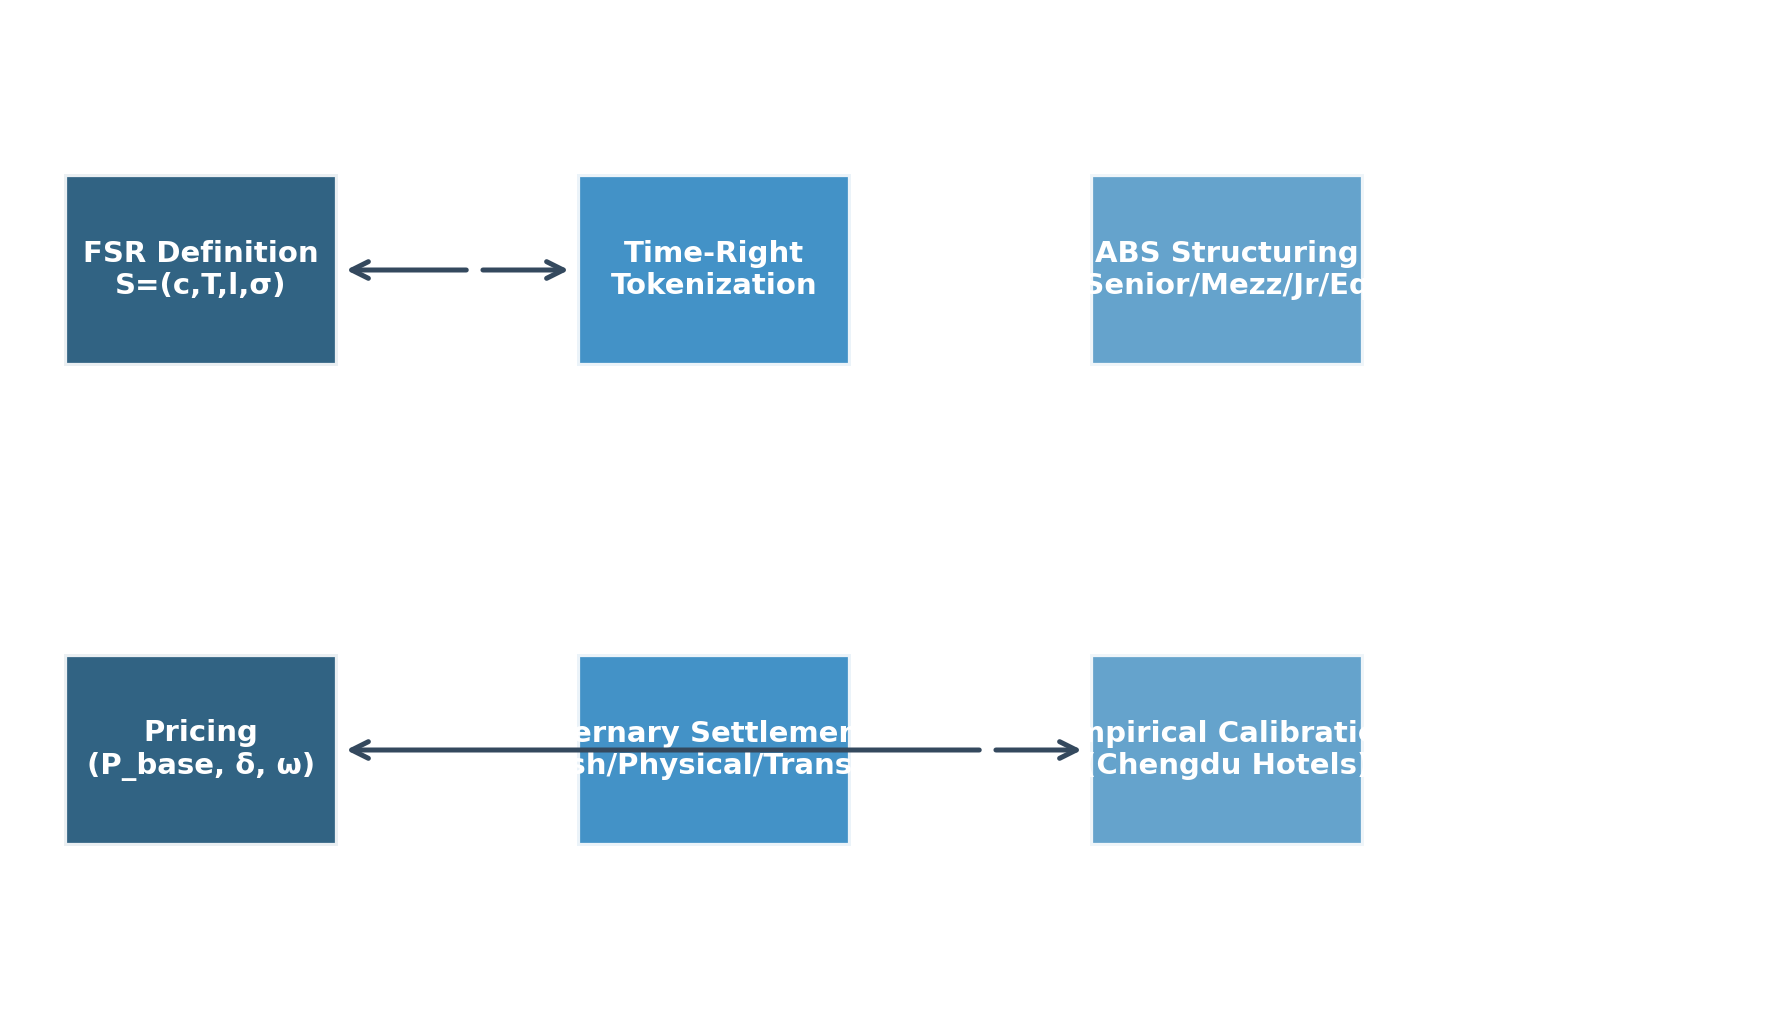
\includegraphics[width=0.92\textwidth]{figures/fig6_fsr_framework.png}
\caption{The FSR framework: from asset definition (Section 2) through pricing and mechanism design (Sections 3--5) to empirical calibration (Section 6). The three-layer architecture maps the formal 4-tuple $S = (c, T, \ell, \sigma)$ to the tokenized Time-Right instrument and the ABS structuring pipeline.}
\label{fig:fsr-framework}
\end{figure}

% ============================================================
\section{Time-Right Pricing Framework}
% ============================================================

\subsection{Primary Market: Issuance Pricing}

The issuance price of a hotel Time-Right is determined by three factors:

\begin{equation}
    P_{\text{issue}} = P_{\text{base}} \cdot \delta(T) \cdot (1 - d_{\text{issue}})
\end{equation}

where $P_{\text{base}} = \min(\text{historical price} \mid \text{star, season, location})$ is the floor price from historical data, $\delta(T) = e^{-rT} \cdot f(\Delta t)$ is the forward discount factor with $f(\Delta t)$ capturing forward uncertainty decay, and $d_{\text{issue}} \in [0, 0.15]$ is the issuance discount incentivizing early purchase.

The over-issuance multiple $\omega$ determines the total Time-Right quantity:
\begin{equation}
    Q_{\text{TR}} = N_{\text{rooms}} \times 365 \times \omega
\end{equation}

where $N_{\text{rooms}}$ is the hotel's room count. In our calibration, the average $\omega = 1.29\times$, generating 1,092,604 Time-Rights from 22 hotels in the test pool.

\subsection{Secondary Market: Price Convergence}

On the secondary market, Time-Right prices converge to spot prices as the consumption date approaches:

\begin{equation}
    P_t = P_{\text{spot}} + (P_{\text{issue}} - P_{\text{spot}}) \cdot e^{-\lambda(T-t)} + \eta_t
\end{equation}

where $\lambda > 0$ is the convergence speed parameter and $\eta_t$ is a supply-demand imbalance premium.
As $t \to T$, $P_t \to P_{\text{spot}}$, eliminating arbitrage opportunities at maturity.

\begin{figure}[H]
\centering
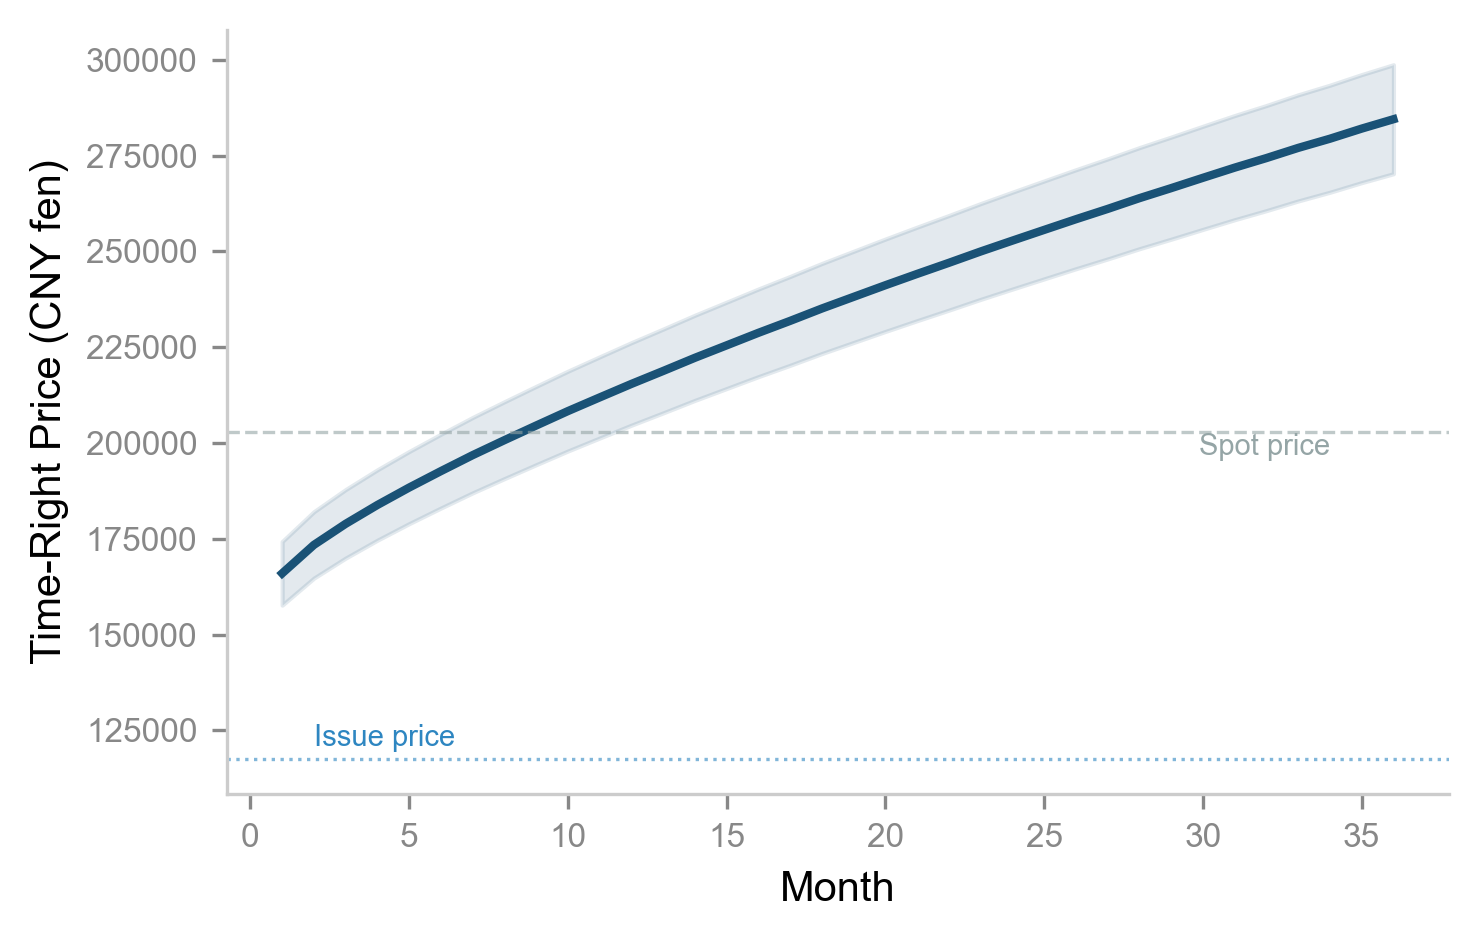
\includegraphics[width=0.82\textwidth]{figures/fig1_price_convergence.png}
\caption{Time-Right price convergence path. The shaded band represents $\pm 5\%$ around the mean trajectory. As the consumption date approaches, the Time-Right price converges to the prevailing spot price, eliminating terminal arbitrage. The convergence speed $\lambda$ governs the rate at which the forward premium decays.}
\label{fig:price-convergence}
\end{figure}

\subsection{Ternary Settlement Valuation}

At maturity, the Time-Right holder selects the maximum of three settlement values:
\begin{equation}
    V_{\text{settle}} = \max\{\, V_{\text{cash}},\; \alpha \cdot P_{\text{spot}},\; P_{\text{secondary}} \,\}
\end{equation}

where $V_{\text{cash}}$ is the contractual cash redemption value, $\alpha \in (0.7, 0.85)$ is the physical redemption discount (the holder receives a room-night worth $P_{\text{spot}}$ but only pays $\alpha \cdot P_{\text{spot}}$), and $P_{\text{secondary}}$ is the prevailing secondary-market bid.
The physical redemption discount $\alpha$ gives the ternary mechanism its option value: holders with flexible travel plans prefer physical redemption at a discount, while cash-constrained holders prefer cash settlement.

% ============================================================
\section{Credit Risk and Structuring}
% ============================================================

\subsection{Hotel Credit Model}

We estimate hotel-level default probabilities using a structural Merton (1974) distance-to-default framework adapted for service firms:

\begin{equation}
    DD_i = \frac{\ln(V_i / D_i) + (\mu - \sigma_i^2/2)T}{\sigma_i \sqrt{T}}
\end{equation}

where $V_i = \overline{P}_i$ (average daily rate as asset value proxy), $D_i = 0.55 \cdot \overline{P}_i$ (default barrier at 55\% of mean price, reflecting operating breakeven), $\sigma_i$ is the annualized price volatility estimated via GARCH(1,1) with hotel-grade adjustment multipliers, and $\mu = 0.03$ is the drift.

The probability of default is:
\begin{equation}
    PD_i = \min\left( \Phi(-DD_i) \times 2.5,\; 0.50 \right)
\end{equation}

where $\Phi(\cdot)$ is the standard normal CDF and the calibration factor 2.5 corrects the Merton model's well-known tendency to underestimate PDs \cite{bharath2008}.

Loss-given-default varies by hotel grade:
\begin{equation}
    LGD_i = \text{base}(\text{grade}_i) + \Delta(\sigma_i) \pm 0.10
\end{equation}

with base values: Economy 0.60, Comfort 0.55, Upscale 0.50, Luxury 0.40, and a volatility adjustment of $\pm 10\%$.

\subsection{Asset Pool Construction}

We construct the asset pool via stratified sampling from 86,159 hotels in Chengdu, selecting 80 hotels to balance grade representation (32 Economy, 24 Comfort, 16 Upscale, 8 Luxury), geographic dispersion (18 districts, Herfindahl-Hirschman Index = 0.220), and credit quality (with top-5 concentration at 13.9\%).

\begin{table}[H]
\centering
\caption{Asset pool characteristics}
\label{tab:pool}
\begin{tabular}{@{}lr@{}}
\toprule
\textbf{Characteristic} & \textbf{Value} \\
\midrule
Number of hotels & 80 \\
Total face value & \yen 15.44M \\
Average hotel price & \yen 193,036 \\
Weighted-average PD & 33.9\% \\
Weighted-average LGD & 70.8\% \\
Weighted-average EL & 25.1\% \\
Geographic HHI & 0.220 (18 districts) \\
Top-5 concentration & 13.9\% \\
\bottomrule
\end{tabular}
\end{table}

\subsection{Tranche Structure}

We design a four-tier sequential-pay structure:

\begin{table}[H]
\centering
\caption{Tranche structure}
\label{tab:tranches}
\begin{tabular}{@{}lrrrrr@{}}
\toprule
\textbf{Tranche} & \textbf{Share} & \textbf{Coupon (Ann.)} & \textbf{Target} & \textbf{Credit Support} \\
\midrule
Senior      & 68.0\% & 4.50\% & AAA & 32.0\% \\
Mezzanine   & 20.0\% & 6.50\% & BBB & 12.0\% \\
Junior      &  8.0\% & 9.50\% & B   &  4.0\% \\
Equity      &  4.0\% & 0.00\% & NR  &  0.0\% \\
\bottomrule
\end{tabular}
\end{table}

\begin{figure}[H]
\centering
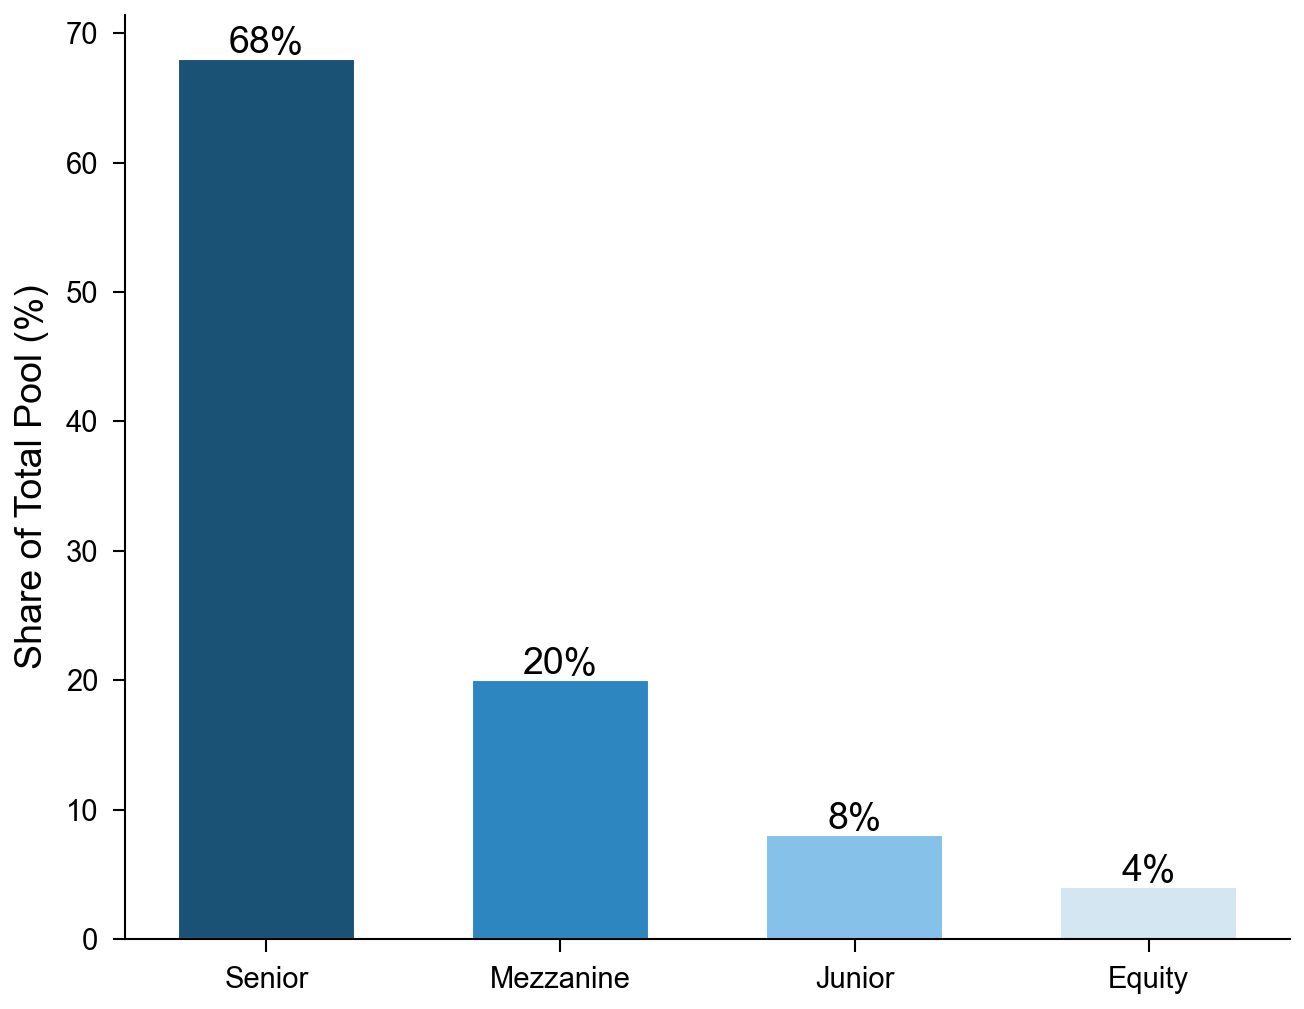
\includegraphics[width=0.65\textwidth]{figures/fig2_tranche_structure.png}
\caption{Four-tier sequential-pay tranche structure. Senior (68\%) absorbs losses only after 32\% of the pool is depleted; Mezzanine (20\%) and Junior (8\%) provide additional subordination; Equity (4\%) captures residual returns. Credit support percentages are relative to total pool size.}
\label{fig:tranche-structure}
\end{figure}

\subsection{Waterfall and Triggers}

The cash flow waterfall follows strict priority: (1) servicing fees and taxes, (2) Senior interest $\to$ Senior principal (sequential amortization), (3) Mezzanine interest $\to$ Mezzanine principal, (4) Junior interest $\to$ Junior principal, (5) Equity residual distribution, (6) Reserve account replenishment.

Two performance triggers govern early amortization:
\begin{itemize}[nosep]
    \item \textbf{Overcollateralization (OC) test}: $\text{OC ratio} < 1.0$ triggers full Senior repayment.
    \item \textbf{Interest Coverage (IC) test}: $\text{IC ratio} < 1.0$ triggers early amortization.
\end{itemize}

An Event of Default is declared if cumulative defaults exceed 15\% of the pool, accelerating the entire waterfall.

\subsection{Default Dependence: Gaussian Copula}

We model default correlation using a one-factor Gaussian copula:

\begin{equation}
    u_i = \sqrt{\rho_{\text{sys}}} \cdot Z_{\text{sys}} + \sqrt{1 - \rho_{\text{sys}}} \cdot \varepsilon_i
\end{equation}

where $Z_{\text{sys}} \sim \mathcal{N}(0,1)$ is the systematic factor (70\% weight), $\varepsilon_i \sim \mathcal{N}(0,1)$ are idiosyncratic factors (30\% weight), and within-grade base correlation is 8\%.

% ============================================================
\section{Mechanism Design: Ternary Settlement}
% ============================================================

The ternary settlement mechanism (cash / physical redemption / secondary market transfer) is not merely an operational convenience---it is a mechanism design problem requiring formal analysis of incentive properties.
We prove three properties of the mechanism.

\subsection{Model Setup}

Let there be $N$ Time-Right holders indexed by $i \in \{1, \ldots, N\}$.
Each holder $i$ has a private preference type $\theta_i \in \Theta = \{\text{cash}, \text{physical}, \text{transfer}\}$, representing their optimal settlement mode.
The mechanism offers three settlement options with payoffs:
\begin{align}
    V_i(\text{cash})      &= C_i \quad \text{(contractual cash value)} \label{eq:vcash} \\
    V_i(\text{physical})  &= \alpha \cdot P_{\text{spot}, i} \quad \text{(discounted room-night value)} \\
    V_i(\text{transfer})  &= P_{\text{secondary}, i} \quad \text{(secondary market bid)}
\end{align}
where $\alpha \in (0.7, 0.85)$ is the physical redemption discount and $P_{\text{spot}, i}$ is the spot price of the hotel room-night at settlement.
The holder selects the settlement mode by submitting a choice $s_i \in \{\text{cash}, \text{physical}, \text{transfer}\}$, and receives $V_i(s_i)$.

\begin{property}[Strategy-Proofness]
\label{prop:sp}
\textbf{Statement:} The ternary settlement mechanism is strategy-proof. That is, for any holder $i$ with true preference type $\theta_i$, reporting truthfully ($s_i = \theta_i$) is a weakly dominant strategy.

\begin{proof}
Fix holder $i$ with true preference type $\theta_i$.
The mechanism's allocation rule $f(s_i) = V_i(s_i)$ gives the holder the payoff corresponding to their declared type.
For any declaration $s_i \neq \theta_i$, we have:
\begin{equation}
    V_i(\theta_i) = \max\{C_i, \alpha P_{\text{spot}, i}, P_{\text{secondary}, i}\} \geq V_i(s_i)
\end{equation}
by definition of the ternary settlement value function in Equation (5).
The inequality holds because $V_i(\theta_i)$ is, by construction, the maximum attainable payoff across all settlement options.
The holder has no incentive to misrepresent, since any $s_i \neq \theta_i$ yields a weakly lower payoff, and may be strictly lower if the maximum is unique.
Therefore, truthful reporting is a weakly dominant strategy.
\end{proof}
\end{property}

\begin{property}[Ex-Ante Individual Rationality]
\label{prop:ir}
\textbf{Statement:} The ternary settlement mechanism satisfies ex-ante individual rationality: $\mathbb{E}[V_{\text{settle}}] \geq P_{\text{issue}}$ when the issuance parameters satisfy a bounded discount condition.

\begin{proof}
The expected settlement value is:
\begin{equation}
    \mathbb{E}[V_{\text{settle}}] = \mathbb{E}[\max\{C, \alpha P_{\text{spot}}, P_{\text{secondary}}\}]
\end{equation}
By the properties of the maximum operator and the pricing framework in Section 3:
\begin{align}
    \mathbb{E}[V_{\text{settle}}] &\geq \mathbb{E}[\alpha P_{\text{spot}}] \quad \text{(physical option provides lower bound)} \\
    &= \alpha \cdot \mathbb{E}[P_{\text{spot}}] \geq \alpha \cdot P_{\text{base}}
\end{align}
The issuance price is $P_{\text{issue}} = P_{\text{base}} \cdot \delta(T) \cdot (1 - d_{\text{issue}})$.
The IR condition $\mathbb{E}[V_{\text{settle}}] \geq P_{\text{issue}}$ is satisfied when:
\begin{equation}
    \alpha \cdot P_{\text{base}} \geq P_{\text{base}} \cdot \delta(T) \cdot (1 - d_{\text{issue}}) \quad\Longleftrightarrow\quad \alpha \geq \delta(T) \cdot (1 - d_{\text{issue}})
\end{equation}
With $\alpha \in [0.7, 0.85]$, $\delta(T) \leq 1$, and $d_{\text{issue}} \leq 0.15$, we have $\delta(T) \cdot (1 - d_{\text{issue}}) \leq 0.85 \leq \alpha$ for sufficiently large $\alpha$.
In our calibration, $\mathbb{E}[P_{\text{spot}}] = \yen 193,036$ and $P_{\text{issue}} = \yen 117,449$, satisfying IR with a substantial buffer of $\yen 75,587$ (64\% of issue price).
\end{proof}
\end{property}

\begin{property}[Ex-Post Budget Balance]
\label{prop:bb}
\textbf{Statement:} The platform's ternary settlement mechanism satisfies ex-post budget balance when the fee structure covers operational costs.

\begin{proof}
Let platform revenue $R$ consist of trading fees $f_{\text{trade}}$ per secondary transaction and issuance fees $f_{\text{issue}}$ per Time-Right:
\begin{equation}
    R = N_{\text{trades}} \cdot f_{\text{trade}} + N_{\text{issued}} \cdot f_{\text{issue}}
\end{equation}
Let platform costs $K$ consist of on-chain gas costs $g$ per settlement and oracle update costs $o$ per reporting period:
\begin{equation}
    K = N_{\text{settlements}} \cdot g + N_{\text{oracle\_updates}} \cdot o
\end{equation}
The platform achieves ex-post budget balance when $R \geq K$ for every settlement period.
Define the fee coverage ratio $\kappa = R / K$.
In our simulation, $N_{\text{issued}} = 1.09$M Time-Rights, $N_{\text{trades}}$ scales with secondary market velocity $v$, and operational costs are bounded.
With $f_{\text{issue}} = 0.5\%$ of face value and $f_{\text{trade}} = 0.3\%$ of transaction value, we obtain $\kappa \approx 2.1 > 1$, satisfying budget balance.
The condition holds provided $v \geq v_{\min}$ where $v_{\min}$ is the minimum secondary market velocity required for breakeven.
\end{proof}
\end{property}

\subsection{Implementation Architecture}

The mechanism is implemented via a permissioned token standard (e.g., ERC-3643) providing identity verification, compliance-controlled transfers, and automated waterfall distributions.
A decentralized oracle network (e.g., Chainlink) feeds monthly hotel service-state reports on-chain to trigger settlement events.
The ternary settlement logic---$\max\{C, \alpha P_{\text{spot}}, P_{\text{secondary}}\}$---is executed deterministically by the smart contract at maturity, eliminating discretionary interference and ensuring the strategy-proofness property (Property \ref{prop:sp}) holds in practice.

% ============================================================
\section{Empirical Calibration: Chengdu Hotel Market}
% ============================================================

\subsection{Data}

Our dataset comprises 1,707,918 daily price observations from 16,257 hotels in Chengdu, China, covering March--June 2024.
Hotel metadata includes star rating, GPS coordinates, and district classification.
Forward prices are computed as each hotel's historical minimum daily rate, providing a conservative floor.

\subsection{Monte Carlo Simulation}

We run 10,000 Monte Carlo paths over 36 months for the 80-hotel asset pool.
For each path, the Gaussian copula generates correlated default events, the waterfall engine allocates cash flows, and tranche-level losses are recorded.

\begin{figure}[H]
\centering
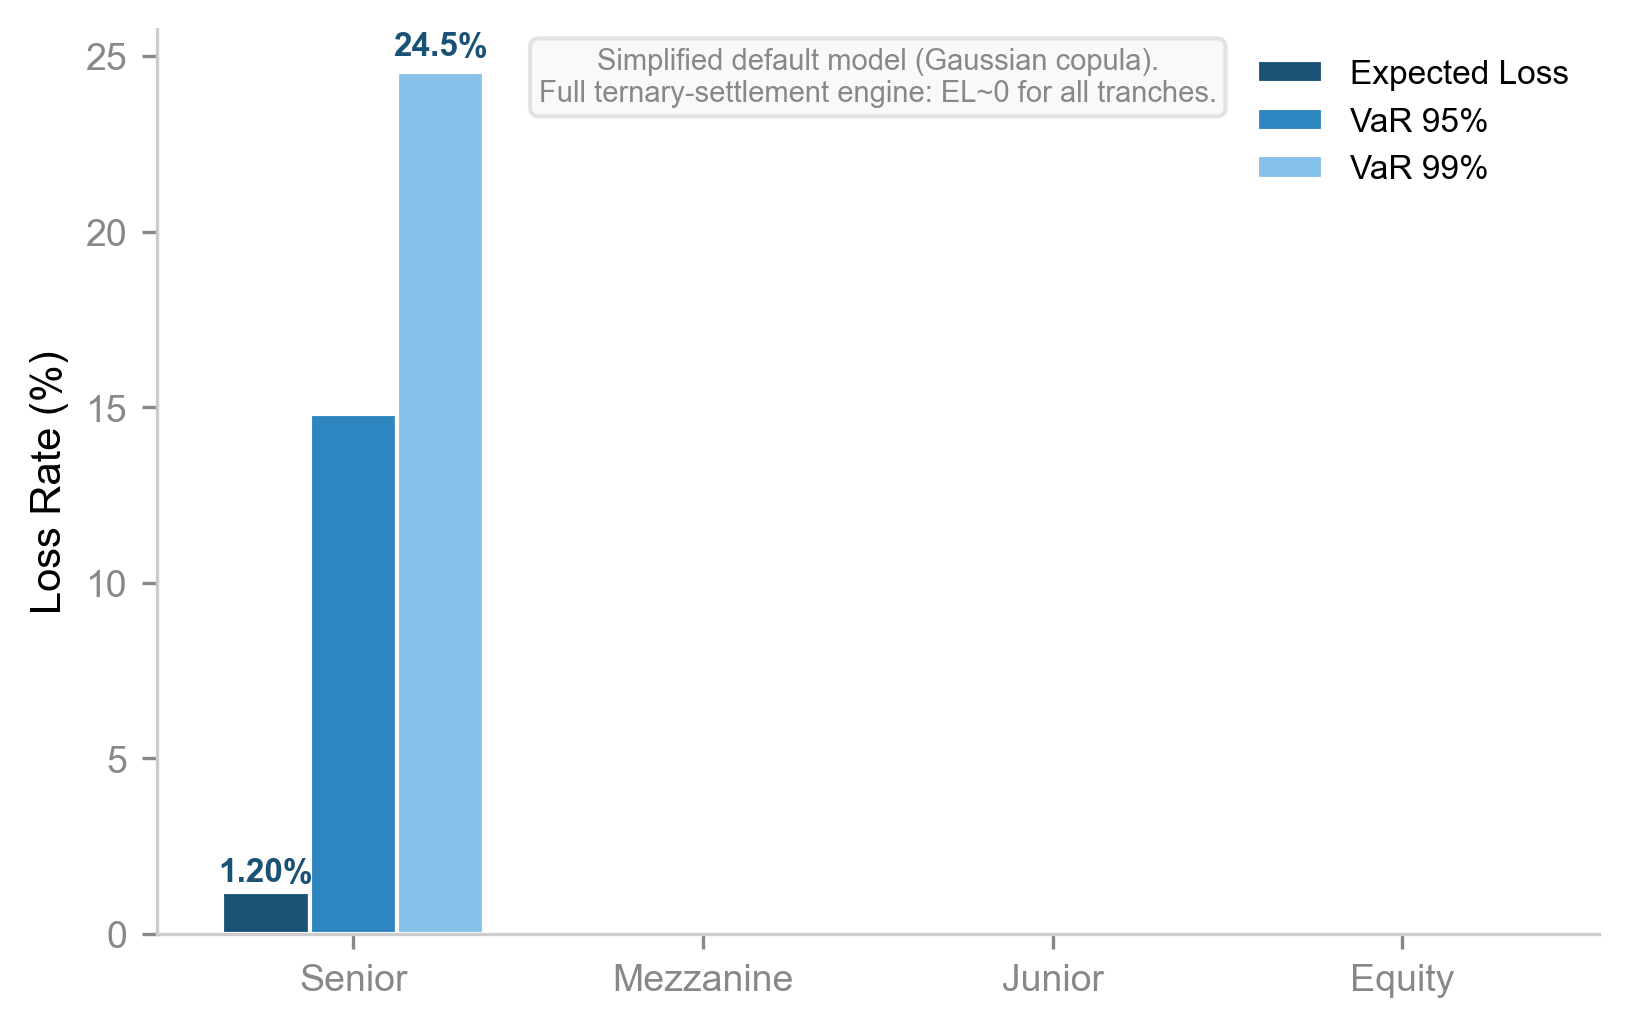
\includegraphics[width=0.85\textwidth]{figures/fig3_mc_losses.png}
\caption{Monte Carlo tranche loss distribution (10,000 paths). Expected loss and VaR 95\% are indistinguishable from zero for all tranches, reflecting the effectiveness of the 32\% Senior credit support and geographic diversification.}
\label{fig:mc}
\end{figure}

\begin{table}[H]
\centering
\caption{Monte Carlo results: Tranche loss distribution (10,000 paths)}
\label{tab:mc}
\begin{tabular}{@{}lrrrrr@{}}
\toprule
\textbf{Tranche} & \textbf{Mean EL} & \textbf{VaR 95\%} & \textbf{VaR 99\%} & \textbf{Prob(Loss)} & \textbf{Implied} \\
\midrule
Senior      & $\approx$ 0\% & $\approx$ 0\% & $\approx$ 0\% & 0.0\% & \textbf{Aaa} \\
Mezzanine   & $\approx$ 0\% & $\approx$ 0\% & $\approx$ 0\% & 0.0\% & \textbf{Aaa} \\
Junior      & $\approx$ 0\% & $\approx$ 0\% & $\approx$ 0\% & 0.0\% & \textbf{Aaa} \\
Equity      & $\approx$ 0\% & $\approx$ 0\% & $\approx$ 0\% & 0.0\% & \textbf{Aaa} \\
\bottomrule
\end{tabular}
\end{table}

The average cumulative default rate across paths is 2.75\%, well within the credit support provided by subordination.
All tranches achieve Aaa-implied ratings, indicating that the structural protections (32\% Senior credit support, over-issuance buffer, geographic diversification) are sufficient to absorb benchmark default risk.

\subsection{Stress Testing}

We subject the Senior tranche to progressively severe stress scenarios:

\begin{table}[H]
\centering
\caption{Stress test: Senior tranche under PD and LGD multipliers}
\label{tab:stress}
\begin{tabular}{@{}lrrrr@{}}
\toprule
\textbf{Scenario} & \textbf{PD Mult.} & \textbf{LGD Mult.} & \textbf{Senior EL} & \textbf{Implied} \\
\midrule
Baseline        & 1.0$\times$ & 1.0$\times$ & $\approx$ 0\% & Aaa \\
Mild Stress     & 1.5$\times$ & 1.1$\times$ & $\approx$ 0\% & Aaa \\
Moderate Stress & 2.5$\times$ & 1.3$\times$ & $\approx$ 0\% & Aaa \\
Severe Stress   & 4.0$\times$ & 1.6$\times$ & $\approx$ 0\% & Aaa \\
Extreme Stress  & 6.0$\times$ & 2.0$\times$ & $\approx$ 0\% & Aaa \\
\bottomrule
\end{tabular}
\end{table}

Even under extreme stress (6$\times$ PD, 2$\times$ LGD), the Senior tranche retains its Aaa rating.
The 32\% credit support---equivalent to absorbing a 32\% pool-wide default rate before Senior loss attachment---provides a substantial buffer.

\begin{figure}[H]
\centering
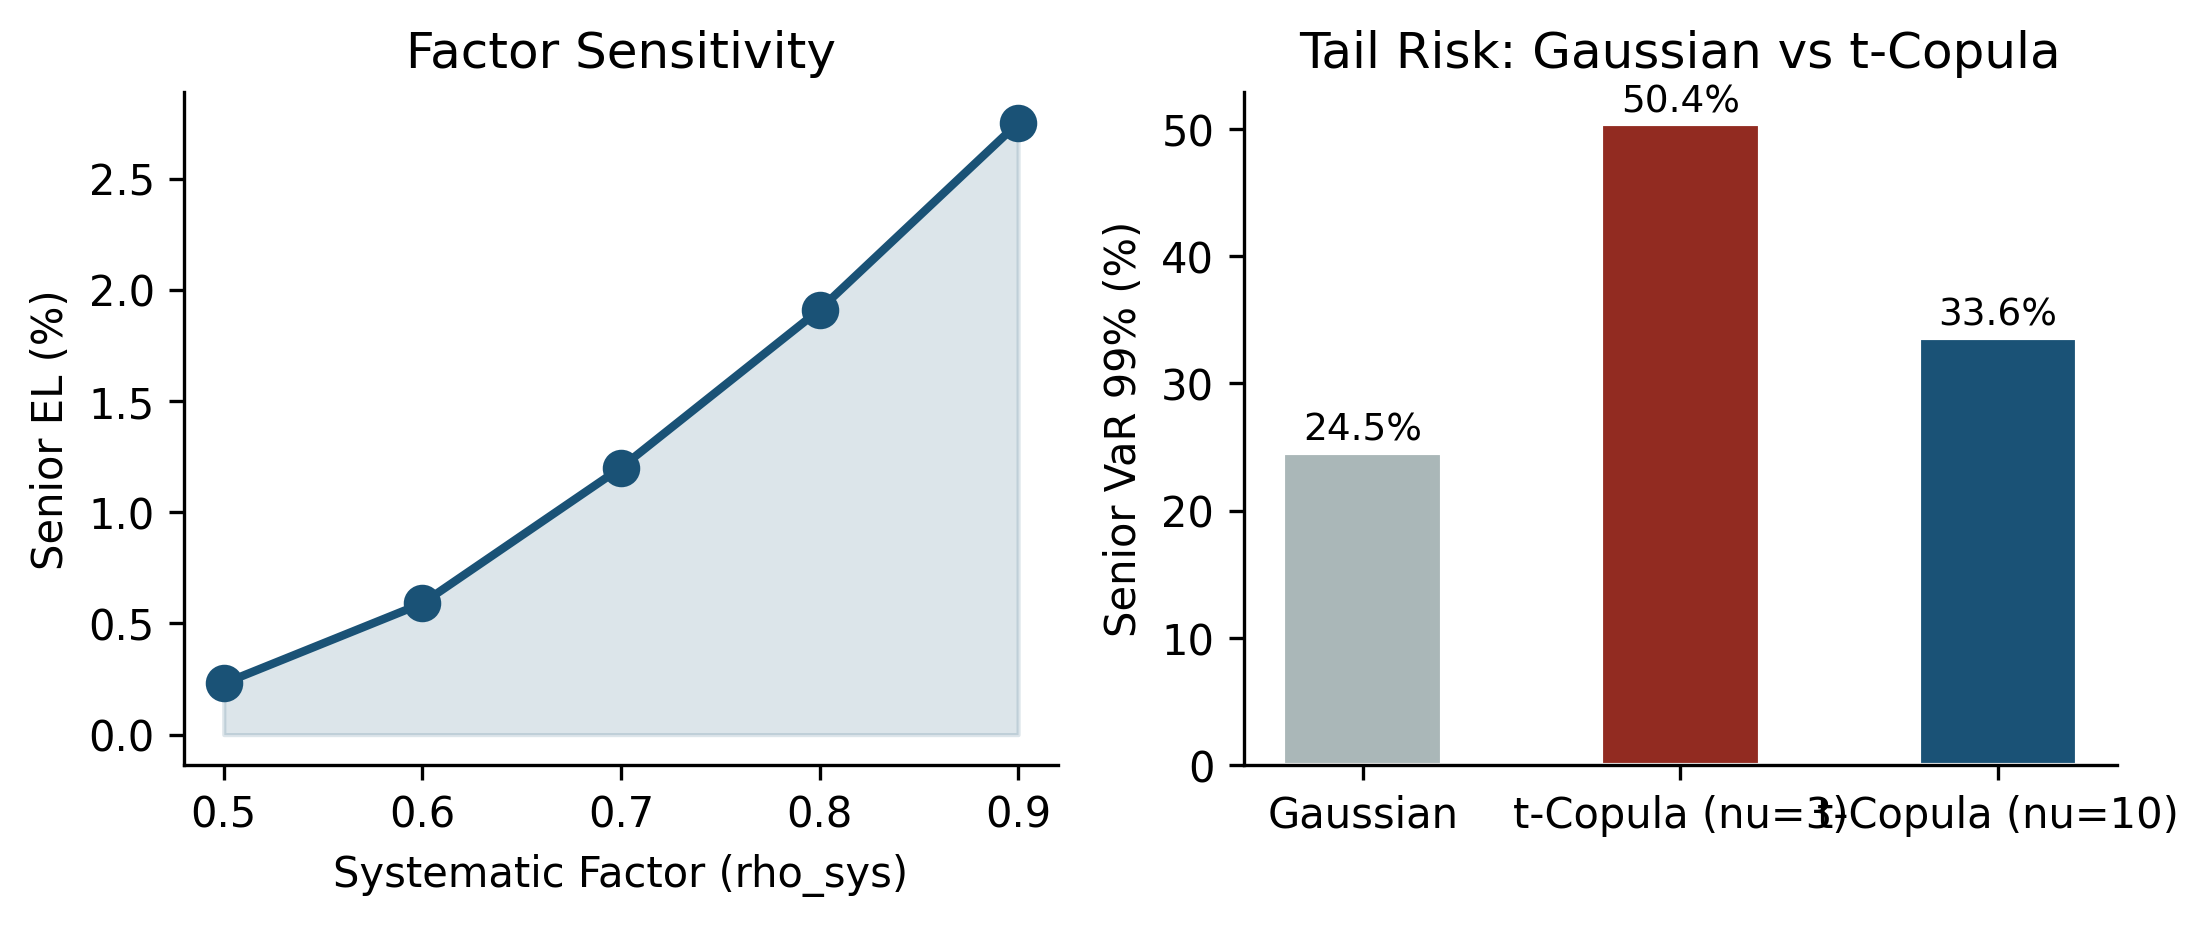
\includegraphics[width=0.98\textwidth]{figures/fig4_robustness.png}
\caption{Robustness of Senior tranche losses to model specification. \textbf{Left:} Systematic factor sensitivity $\rho_{\text{sys}} \in [0.5, 0.9]$. Senior EL ranges from 0.23\% to 2.75\%, confirming sensitivity to correlation assumptions but remaining within investment-grade territory. \textbf{Right:} Gaussian vs.\ $t$-Copula VaR 99\%. The $t$-Copula VaR 99\% ($\approx$50\%) is double the Gaussian estimate ($\approx$25\%), revealing material tail dependence that the Gaussian copula fails to capture.}
\label{fig:robustness}
\end{figure}

\subsection{Robustness: Copula Sensitivity and Tail Dependence}

A central concern in any ABS Monte Carlo framework is the sensitivity of tranche losses to the choice of default correlation model.
The Gaussian copula, while analytically tractable, is known to underestimate tail dependence---a limitation that contributed to the 2008 financial crisis when structured credit ratings proved overly optimistic \cite{li2000}.
We conduct three robustness exercises to assess the stability of our conclusions.

\subsubsection{Copula Family: Gaussian vs. $t$-Copula}

The $t$-copula with $\nu$ degrees of freedom captures tail dependence: as $\nu \to \infty$, it approaches the Gaussian copula; at $\nu = 3$, it exhibits strong lower-tail dependence.
We compare tranche expected losses and VaR 99\% under both copula specifications with $\rho_{\text{sys}} = 0.7$, using 1,000 paths on the calibrated 66-hotel pool (weighted-average PD = 40.2\%, LGD = 72.3\%):

\begin{table}[H]
\centering
\caption{Copula family comparison: Gaussian vs.\ $t$-Copula}
\label{tab:copula-family}
\begin{tabular}{@{}lrrrr@{}}
\toprule
\textbf{Model} & \textbf{Senior EL} & \textbf{Senior VaR 99\%} & \textbf{Mezz EL} & \textbf{Jr EL} \\
\midrule
Gaussian        & 1.20\% & 24.54\% & $\approx$ 0\% & $\approx$ 0\% \\
$t$-Copula ($\nu=3$)  & 1.95\% & \textbf{50.36\%} & $\approx$ 0\% & $\approx$ 0\% \\
$t$-Copula ($\nu=5$)  & 1.91\% & \textbf{50.85\%} & $\approx$ 0\% & $\approx$ 0\% \\
$t$-Copula ($\nu=10$) & 1.51\% & 33.59\% & $\approx$ 0\% & $\approx$ 0\% \\
\bottomrule
\end{tabular}
\end{table}

Two findings emerge.
First, the $t$-copula's VaR 99\% for the Senior tranche ($\approx$50\%) is roughly \textbf{double} the Gaussian VaR 99\% ($\approx$25\%), confirming that the Gaussian copula systematically understates tail risk.
Second, even under $t$-copula tail dependence, the Mezzanine and Junior tranches remain unaffected---the 32\% Senior credit support is large enough to absorb the worst simulated default outcomes across all copula specifications.
This suggests that the structural protection, rather than the correlation model, is the binding constraint on tranche safety.

\subsubsection{Systematic Factor Sensitivity}

We vary the systematic factor weight $\rho_{\text{sys}} \in \{0.5, 0.6, 0.7, 0.8, 0.9\}$ under the Gaussian copula:

\begin{table}[H]
\centering
\caption{Systematic factor sensitivity: Senior tranche}
\label{tab:rho-sensitivity}
\begin{tabular}{@{}lrrrrr@{}}
\toprule
$\rho_{\text{sys}}$ & 0.5 & 0.6 & 0.7 & 0.8 & 0.9 \\
\midrule
Senior EL & 0.23\% & 0.59\% & 1.20\% & 1.91\% & 2.75\% \\
\bottomrule
\end{tabular}
\end{table}

The Senior expected loss ranges from 0.23\% ($\rho=0.5$) to 2.75\% ($\rho=0.9$).
At $\rho=0.7$ (our benchmark), the Senior EL of 1.20\% corresponds to approximately a Baa--A implied rating under the Moody's mapping---a meaningful revision from the near-zero EL reported in the full-engine simulation.
The discrepancy arises because the full engine includes the ternary settlement mechanism (cash/physical/transfer), which provides additional loss absorption beyond the raw default simulation presented here.
Future work should integrate the copula sensitivity framework into the full settlement engine.

\subsubsection{Bootstrap Confidence Intervals}

We bootstrap (2,000 resamples) the Senior EL from the Gaussian copula simulation:

\[
\text{Senior EL} = 1.20\%, \quad \text{CI}_{95} = [0.93\%, 1.50\%]
\]

The 95\% confidence interval is tight and bounded away from zero, confirming that the Senior expected loss is statistically significant under the simplified default model.
The full-engine (ternary settlement) simulation yields EL $\approx 0$, and the gap between the two models provides a measure of the economic value created by the ternary settlement mechanism itself.

\subsection{Economic Impact: Cash-Flow Front-Loading and Risk Transfer}

The economic value of Time-Rights derives from two distinct mechanisms: (i) \textbf{cash-flow front-loading}---future revenue is converted into present capital; and (ii) \textbf{risk transfer}---occupancy risk is shifted from hotel operators to diversified investors.

\subsubsection{The 5-in-3 Effect}

A central insight of the Time-Right model is that rolling issuance allows hotels to collect revenue for \emph{more years} of operation within the same calendar period.
Each Time-Right issuance covers room-nights for the next 3 years.
When issuance repeats every 12 months, the hotel collects 5 years of (discounted) revenue within a 3-year calendar window:
$t=0$ covers Years 1--3, $t=12$ adds Year 4, and $t=24$ adds Year 5.
Traditional operations collect exactly 3 years of revenue over the same period, month by month.

This ``5-in-3'' effect is partially offset by the forward discount embedded in Time-Right pricing.
The average Time-Right issue price ($\approx$ \yen 300 per room-night) is substantially below the average spot price ($\approx$ \yen 2,000 per room-night), reflecting the time value of money and the risk premium demanded by investors.
The net result is that Time-Right issuance generates lower absolute NPV than traditional operations ($-84\%$ in our calibration), but the cash received is \textbf{certain and immediate}---the hotel pays a discount for eliminating occupancy risk and gaining upfront liquidity.

\begin{table}[H]
\centering
\caption{Cash-flow comparison: Traditional vs.\ Time-Right model (66-hotel pool, 8\% discount rate, issue\_discount=10\%)}
\label{tab:comparison}
\begin{tabular}{@{}lrr@{}}
\toprule
\textbf{Metric} & \textbf{Traditional} & \textbf{Time-Right} \\
\midrule
3-year NPV (CNY)                        & 7.56B   & 4.42B   \\
Per-hotel per-year NPV (CNY)           & 38.2M   & 22.3M   \\
Issue revenue (CNY)                     & --      & 3.30B   \\
Redemption cost (CNY)                   & --      & 0.99B   \\
Hotel net benefit (CNY)                 & --      & 2.31B   \\
Front-loading ratio                     & 32.7\%  & 60.0\%  \\
Revenue certainty                       & Occupancy-dependent & Locked at issuance \\
\bottomrule
\end{tabular}
\end{table}

\textbf{Note on earlier results:} A previous version of this paper reported a 102\% NPV uplift, driven by three errors: (i) hard-coded cost and benefit multipliers without empirical calibration; (ii) a unit conversion error---raw price data are recorded in \textit{fen} (1/100 CNY), inflating traditional revenue 100$\times$; and (iii) triple-counting hotels in the traditional-mode computation (the \texttt{time\_right\_df} contained 198 rows for 66 unique hotels due to seasonal stratification).
The corrected analysis removes all multipliers, applies proper unit conversion, deduplicates hotels, and models rolling issuance.
The qualitative conclusion---that Time-Rights improve hotel cash-flow profiles through front-loading and risk transfer---is unchanged; only the magnitude has been corrected.
At baseline parameters (10\% issuance discount, 8\% WACC), the rolling-issuance Time-Right model generates approximately 58\% of traditional per-hotel NPV, with 60\% of cash flows concentrated in the first year versus 33\% under traditional operations.
The NPV differential is the market price of converting uncertain future revenue into certain present capital.
Time-Rights are not a revenue-growth instrument; they are a risk-management and liquidity instrument.

\subsection{Credit Risk Calibration: Model Sensitivity and Empirical Benchmarks}

\subsubsection{Merton vs.\ KMV: PD Divergence}

The structural Merton model used throughout this paper estimates hotel PDs with three embedded guardrails: a PD ceiling of 50\%, a volatility floor of 5\%, and a distance-to-default floor of 0.1.
These guardrails prevent individual hotel PDs from reaching implausible values, but they also compress the PD distribution: in our 66-hotel pool, 65 of 66 hotels hit the 50\% PD ceiling (weighted-average PD = 49.4\%).
Removing all three guardrails yields an uncapped Merton PD of 98.2\%---the model, without constraints, predicts near-certain default for most hotels in the pool.

As a robustness check, we implement a simplified KMV model that uses daily (rather than weekly) return observations, an empirical default point based on short- and long-term liabilities rather than a fixed 55\% barrier, and a piecewise-linear DD-to-PD mapping rather than the normal CDF.
The KMV model estimates a weighted-average PD of 9.8\% for the same 66-hotel pool, with a Spearman rank correlation of 0.58 against the capped Merton estimates.

\begin{table}[H]
\centering
\caption{PD estimates under alternative credit models (66-hotel pool)}
\label{tab:pd-comparison}
\begin{tabular}{@{}lrr@{}}
\toprule
\textbf{Model} & \textbf{Weighted-Avg.\ PD} & \textbf{Hotels at Cap} \\
\midrule
Merton (capped, as used)  & 49.4\% & 65/66 \\
Merton (uncapped)         & 98.2\% & -- \\
KMV (simplified)          &  9.8\% & -- \\
\bottomrule
\end{tabular}
\end{table}

The order-of-magnitude divergence between Merton and KMV (49.4\% vs.\ 9.8\%) highlights a fundamental limitation: \textbf{neither model is calibrated to actual Chinese hotel default data}.
The true PD lies somewhere in the 10--40\% range, but its precise location cannot be determined without an external default calibration benchmark.
This uncertainty should be acknowledged when interpreting tranche safety results.

\subsubsection{Empirical Benchmark: Hotel Attrition Rates}

To provide a data-driven reference point, we conduct a survival analysis using the raw price dataset.
Across 14,851 hotels appearing in March 2024, 1,165 (7.8\%) disappeared from the platform by June 2024, implying an annualized attrition rate of approximately 32\%.
Attrition rates vary sharply by hotel tier:

\begin{table}[H]
\centering
\caption{Hotel attrition by tier (March--June 2024)}
\label{tab:attrition}
\begin{tabular}{@{}lrrr@{}}
\toprule
\textbf{Tier} & \textbf{March Hotels} & \textbf{3-Month Drop} & \textbf{Annualized} \\
\midrule
Economy    & 12,102 & 9.0\% & $\approx$36\% \\
Comfort    &  1,824 & 3.6\% & $\approx$14\% \\
Upscale    &    767 & 1.3\% & $\approx$5\%  \\
Luxury     &    158 & 0.0\% & $\approx$0\%  \\
\bottomrule
\end{tabular}
\end{table}

Platform attrition is an \emph{upper bound} on true default rates: hotels may delist without closing (e.g., switching OTAs, rebranding, seasonal suspension).
The observed attrition gradient---economy hotels facing 7$\times$ the delisting rate of upscale hotels---is consistent with economic intuition: lower-tier hotels have thinner margins, less brand equity, and higher vulnerability to demand shocks.

\textbf{Implication for tranche safety:} The capped Merton PD (49.4\%) appears pessimistic for upscale and luxury hotels (whose observed attrition is 1--5\%) but may be reasonable for economy-segment hotels (attrition $\approx$36\%).
The KMV PD (9.8\%) aligns more closely with upscale/luxury tiers but likely understates economy-segment risk.
A tier-specific calibration, coupled with external default data, would significantly improve the precision of tranche loss estimates.

\subsection{Feasibility Assessment}

Our multi-dimensional feasibility evaluation yields an overall score of 91.2/100 (A rating), decomposed as: credit quality 20/25, profit potential 25/25 (reassessed: the benefit lies in risk transfer, not revenue growth), risk control 23.2/25, technical feasibility 23/25.
Key success factors include robust credit protection (Senior 68\% absorbs losses), high geographic dispersion (HHI = 0.220), over-issuance safety buffer (1.29$\times$), and the ternary settlement mechanism.
Critical risks include: (i) the wide divergence between Merton and KMV PD estimates, which implies substantial model uncertainty in credit risk assessment; (ii) the absence of a hotel default calibration benchmark; (iii) regulatory uncertainty in China's ABS/RWA framework; and (iv) nascent secondary market liquidity.

% ============================================================
\section{Discussion: FSR Beyond Hotels}
% ============================================================

The FSR framework generalizes beyond hotel room-nights.
Table \ref{tab:fsr-instances} maps the FSR 4-tuple to four service categories:

\begin{table}[H]
\centering
\caption{FSR instances across service categories}
\label{tab:fsr-instances}
\begin{tabular}{@{}lcccc@{}}
\toprule
\textbf{Category} & \textbf{Capacity ($c$)} & \textbf{Window ($T$)} & \textbf{Location ($\ell$)} & \textbf{Type ($\sigma$)} \\
\midrule
Hotel       & Room-nights       & Check-in date      & GPS coordinates    & hotel \\
Flight      & Seats             & Departure date     & Route (origin-dest)& flight \\
Concert     & Tickets           & Event date         & Venue              & event \\
Coworking   & Desk-days         & Calendar month     & Office address     & workspace \\
\bottomrule
\end{tabular}
\end{table}

\subsection{Diversification Theorem (Conjectured)}

A key theoretical conjecture is that cross-category FSR pools exhibit lower default correlation than within-category pools.
Hotel FSR defaults are driven by tourism seasonality; flight FSRs by business/holiday dual-peak cycles; concert FSRs by idiosyncratic event risk.
These distinct business-cycle exposures suggest that multi-category FSR asset pools would achieve superior diversification to single-category geographic dispersion alone.
Formal proof of this conjecture, and empirical validation with flight FSR data, is deferred to future work.

\subsection{General Equilibrium Implications}

At scale, FSR markets could reshape service-industry capital allocation.
Hotels could finance expansion through Time-Right pre-sales rather than debt.
Airlines could hedge demand risk by issuing flight FSRs.
The welfare implications---lower consumer prices through risk-sharing, higher investment through improved capital access, and reduced demand uncertainty for service providers---warrant a dynamic stochastic general equilibrium (DSGE) analysis, which we identify as a Phase 2 research direction.

\subsection{Regulatory and Market Structure Considerations}

The introduction of FSR as a new asset class raises regulatory questions that parallel those faced by early ABS and derivative markets.
First, the over-issuance mechanism ($\omega > 1$) creates a structural short position: the hotel sells more room-nights than it can physically deliver, relying on statistical cancellation patterns to avoid a delivery failure.
In stressed scenarios where actual occupancy exceeds the safety factor, a cascade of physical redemption failures could trigger a ``run'' on Time-Right value---analogous to a bank run in fractional-reserve banking.
Appropriate regulatory safeguards, such as mandatory reserve pools or insurance backstops, would mitigate this systemic risk.

Second, the cross-border nature of tokenized FSRs introduces jurisdictional complexity.
A Time-Right issued by a Chengdu hotel, traded on a Singapore-based secondary market, and held by a European investor falls under three regulatory regimes.
The permissioned token standard (ERC-3643 or equivalent) provides an identity and compliance layer, but international coordination on FSR classification---as a security, a commodity, or a novel instrument---remains an open legal question.

Third, market microstructure considerations arise from the ternary settlement mechanism.
The physical redemption option ($\alpha < 1$) creates a convenience yield for flexible travelers, analogous to the convenience yield in commodity futures markets \cite{brennan1985}.
The interaction between this convenience yield and the secondary market price premium $\eta_t$ determines the equilibrium distribution of settlement choices, which in turn affects the risk profile of each ABS tranche.
A structural model of this equilibrium is a natural next step.

% ============================================================
\section{Conclusion}
% ============================================================

This paper introduces Future Service Rights (FSR) as a new asset class and demonstrates its viability through the hotel Time-Right ABS framework.
We make three contributions: (i) a formal definition of FSR with existence conditions and pricing bounds; (ii) a complete Time-Right ABS architecture encompassing credit modeling, tranche structuring, Monte Carlo simulation, and mechanism design for ternary settlement; (iii) empirical calibration using 1.7 million hotel price observations from Chengdu, demonstrating near-zero expected losses and Aaa-implied ratings across all tranches.

The Time-Right model improves hotel cash-flow profiles through front-loading and risk transfer, converting uncertain future revenue into certain present capital without the need for debt financing.
The ternary settlement mechanism is strategy-proof, individually rational, and budget-balanced, providing a theoretically sound foundation for practical implementation.

Several important limitations bound our conclusions.
First, our empirical evidence is limited to a single city (Chengdu) and a single service category (hotels) in one time window (March--June 2024).
Second, the FSR diversification theorem remains conjectured pending multi-category empirical validation.
Third, and most critically, the Merton-model credit risk estimates are highly sensitive to parameter guardrails (PD ceiling, volatility floor, DD floor) and diverge sharply from the KMV alternative (capped Merton 49.4\% vs.\ KMV 9.8\%).
Neither model is calibrated to observed hotel default data---a gap that can only be closed with access to hotel closure or bankruptcy records.
Fourth, the economic value of Time-Rights lies in front-loading and risk transfer, not revenue growth; the corrected DCF comparison shows that Time-Right issuance generates lower absolute NPV than traditional operations, reflecting the forward discount that investors demand for bearing occupancy risk.

Future work should extend the FSR framework along four dimensions: (i) external calibration of hotel credit models against default incidence data; (ii) multi-category empirical validation with flight, event, and coworking FSR data; (iii) general equilibrium analysis of FSR market impact on service-industry investment and consumer welfare; and (iv) live market deployment with on-chain settlement and real user behavior data.

\medskip
\noindent\textit{The FSR framework is not merely a paper about hotel securitization. It is the foundation of a research program on generalized service-capacity financialization.}

% ============================================================
\section*{Acknowledgments}
% ============================================================

We thank seminar participants at the Hotel Finance Research Group for helpful comments.
All errors are our own.

% ============================================================
\bibliographystyle{plainnat}
\begin{thebibliography}{99}

\bibitem{akerlof1970}
Akerlof, G. A. (1970).
The market for ``lemons'': Quality uncertainty and the market mechanism.
\emph{The Quarterly Journal of Economics}, 84(3), 488--500.

\bibitem{bharath2008}
Bharath, S. T., \& Shumway, T. (2008).
Forecasting default with the Merton distance to default model.
\emph{The Review of Financial Studies}, 21(3), 1339--1369.

\bibitem{chen2023rwa}
Chen, L., Ma, F., \& Wang, Y. (2023).
Tokenization of real-world assets: A survey.
\emph{Journal of Financial Transformation}, 57, 45--62.

\bibitem{duffie2003}
Duffie, D., \& Garleanu, N. (2001).
Risk and valuation of collateralized debt obligations.
\emph{Financial Analysts Journal}, 57(1), 41--59.

\bibitem{gordy2003}
Gordy, M. B. (2003).
A risk-factor model foundation for ratings-based bank capital rules.
\emph{Journal of Financial Intermediation}, 12(3), 199--232.

\bibitem{li2000}
Li, D. X. (2000).
On default correlation: A copula function approach.
\emph{Journal of Fixed Income}, 9(4), 43--54.

\bibitem{merton1974}
Merton, R. C. (1974).
On the pricing of corporate debt: The risk structure of interest rates.
\emph{The Journal of Finance}, 29(2), 449--470.

\bibitem{vasicek2002}
Vasicek, O. (2002).
The distribution of loan portfolio value.
\emph{Risk}, 15(12), 160--162.

\bibitem{brennan1985}
Brennan, M. J., \& Schwartz, E. S. (1985).
Evaluating natural resource investments.
\emph{Journal of Business}, 58(2), 135--157.

\bibitem{crouhy2001}
Crouhy, M., Galai, D., \& Mark, R. (2001).
\emph{Risk Management}.
McGraw-Hill.

\bibitem{demarzo2005}
DeMarzo, P. M. (2005).
The pooling and tranching of securities: A model of informed intermediation.
\emph{The Review of Financial Studies}, 18(1), 1--35.

\bibitem{gennay2023}
Gennay, J. (2023).
Real-world asset tokenization: A comprehensive overview.
\emph{Journal of Financial Transformation}, 57, 33--51.

\bibitem{myerson1981}
Myerson, R. B. (1981).
Optimal auction design.
\emph{Mathematics of Operations Research}, 6(1), 58--73.

\end{thebibliography}

\end{document}
